\section{Derivatives and Integrals of Vector Functions}
\begin{definition}[Derivative of a Vectoe Function]
    For a vector function \(\vec{r}(t)=\langle f(t),g(t),h(t) \rangle,t\in\R \), we define
    \[
        \vec{r}\,^{\prime} =\lim_{h \to0} \frac{\vec{r}(t+h)-\vec{r}(t)}{h}
    \]
    provided this limit exists.
\end{definition}
From our earlier definition of the limit of a vector function, we have
\[ 
   \lim_{h\to0} \frac{\vec{r}(t+h)-\vec{r}(t)}{h}=\left\langle \lim_{h\to 0}\frac{f(t+h)-f(t)}{h},\lim_{h\to 0}\frac{g(t+h)-g(t)}{h},\lim_{h\to 0}\frac{h(t+h)-h(t)}{h} \right\rangle
\]
We call this vector the \textbf{tangent vector}.\\
For example, consider the following space curve: 
\begin{center}
    \[
        \vec{r}(t)=\left\langle t\cos (t),t,t\sin (t) \right\rangle 
    \]
    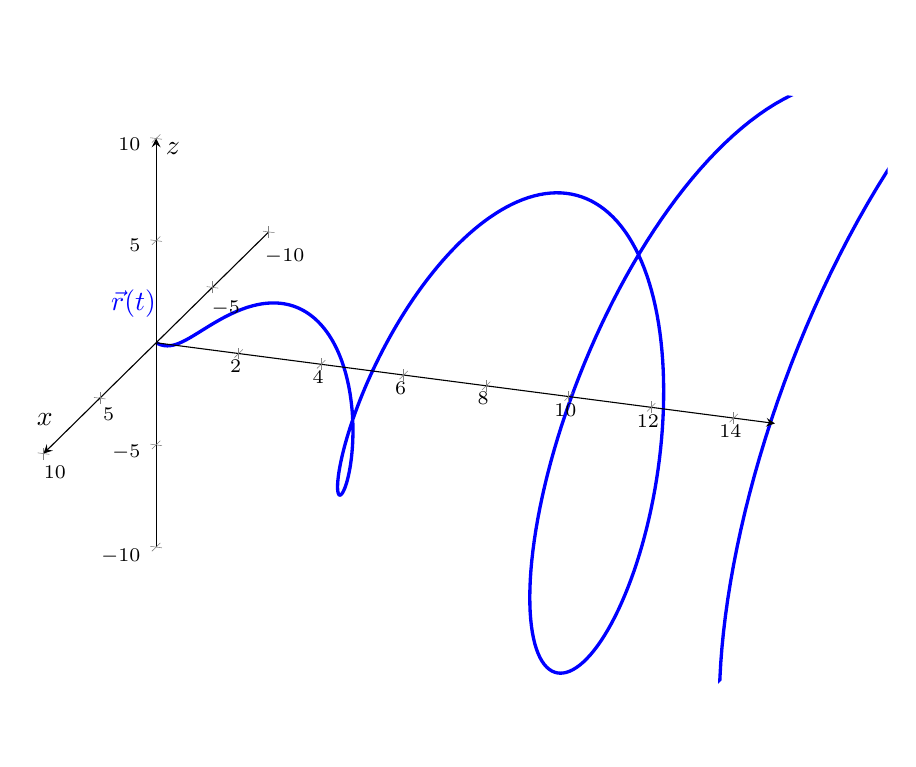
\begin{tikzpicture}
        \begin{axis}[
            width=2*175pt,
			tick label style={font=\scriptsize},
			axis on top,
			view={110}{30},
			axis lines=center,
			name=3dplot,
			ymin=0, ymax=15, xmin=-10, xmax=10, zmin=-10, zmax=10,
			xlabel=$x$, ylabel=, zlabel=$z$]
            \addplot3[samples=600, samples y=0, domain=0:25, domain y=0:25, color=blue, very thick] ({x*cos(deg(x))},{x},{x*sin(deg(x))});
            \node[color=blue] at (2,0,3) {\(\vec{r}(t)\)};
        \end{axis}
    \end{tikzpicture}
\end{center}
We give
\[
    \vec{r}^{\prime} (t)=\left\langle \cos (t)-t\sin (t),1,\sin (t)+t\cos (t) \right\rangle 
\]
\begin{definition}[Tangent Line]
    The tangent line to the curve traced by \(\vec{r}(t)\) at point \(P=(x_0,y_0,z_0)\) is the line parallel to the tangent vector and through point \(P\). We give the following definition: 
    \[
        \frac{x-x_0}{f^{\prime} (t)}=\frac{y-y_0}{g^{\prime} (t)}=\frac{z-z_0}{h^{\prime} (t)}
    \]
\end{definition}
\begin{definition}[Unit Tangent Vector]
    We often use the \textbf{Unit Tangent Vector}, \(\vec{T}(t)\) , where
    \[
        \vec{T}(t)=\frac{\vec{r}\,^{\prime} (t)}{|\vec{r}\,^{\prime} (t)|}
    \]
\end{definition}
Example: find the unit tangent vector at \(t=0\) for
\[
    \vec{r}(t)=t^3 e^t\hati-4t^3\hatj+\sin (3t)\hatk
\]
\[
    \vec{r}\,^{\prime} (t)=(3t^2 e^{t+t^3 e^t} )\hati-12t^2 \hatj+3\cos (3t)\hatk
\]
\[
    \Longrightarrow \vec{r}\,^{\prime} (0)=3\hatk
\]
If we changed the \(\hatk\) component to \(\cos \) instead of \(\sin \), we would have \(\vec{r}\,^{\prime} (0)=\vec{0}\), meaning the derivative is undefined for \(t=0\).\\
\begin{definition}[Differentiation Rules for Vector-Valued Functions]
    Let \(\vec{v}(t),\vec{u}(t)\) be differentiable vector functions, \(c\in\mathbb{R} \) , and \(f\) is a real-valued function.
    \begin{itemize}
        \item \(\frac{d}{dt}(\vec{u}(t)+\vec{v}(t))=\frac{d}{dt}\vec{u}(t)+\frac{d}{dt}\vec{v}(t)\) 
        \item \(\frac{d}{dt}(c\vec{u}(t))=c\vec{u}\,^{\prime} (t)\)
        \item \(\frac{d}{dt}(f(t)\vec{u}(t))=f(t)\vec{u}\,^{\prime} (t)+f^{\prime} (t)\vec{u}(t)\) 
        \item \(\frac{d}{dt}(\vec{v}(t)\cdot\vec{u}(t))=\vec{u}\,^{\prime} (t)\cdot\vec{v}(t)+\vec{v}\,^{\prime} (t)\cdot\vec{u}(t)\) 
        \item \(\frac{d}{dt}(\vec{u}(t)\times \vec{v}(t))=\vec{u}\,^{\prime} (t)\times \vec{v}(t)+\vec{u}(t)\times \vec{v}\,^{\prime} (t)\) 
        \item \(\frac{d}{dt}\vec{u}(f(t))=f^{\prime} (t)\vec{u}\,^{\prime} (f(t))\)
    \end{itemize}
    For all of these, order of operation will only matter for the cross product.
\end{definition}
\begin{definition}[Integrals of Vector Functions]
    For \(t\in I=[\alpha,\beta] \subseteq\mathbb{R} \) we give
    \[
        \int_I \vec{r}(t)dt=\left\langle \int_\alpha^\beta f(t)dt,\int_\alpha^\beta g(t),\int_\alpha^\beta h(t) \right\rangle +\vec{C}
    \]
\end{definition}
\section{Arc Length and Curvature}
\begin{definition}[Arclength Function \(s\) in 3 Dimensions]
    For \(\vec{r}(t)=\left\langle f(t),g(t),h(t) \right\rangle,t\in[a,b]\subseteq \mathbb{R}  \), we have
    \[
        s(t)=\int _a^t \left|\vec{r}\,^{\prime} (u)\right|du=\int_a^t \sqrt{\left( \frac{dx}{du} \right)^{2}+\left( \frac{dy}{du} \right)^2 +\left( \frac{dz}{du} \right)^2    }du  
    \]
\end{definition}
\begin{definition}[Smooth Parametrization of a Curve]
    \(\vec{r}(t)\) is smooth for an interval \(t\in I\)  if \(\vec{r}\,^{\prime} \) is continuous and \(\vec{r}\,^{\prime} (t)\neq \vec{0} \forall t\in I\). 
\end{definition}
\begin{definition}[Curvature (The intuitive and useless definition)]
\[
    \kappa =\left\vert \frac{d\vec{T}}{ds} \right\vert
\]
\end{definition}
Suppose we have \(\left|\vec{r}(t)\right| = c\in\mathbb{R} \forall t\). We then have
\[
    \vec{r}(t)\cdot\vec{r}(t)=\left|\vec{r}(t)\right|^2=c^2
\]
\[
    \Longrightarrow \frac{d\vec{r}}{dt}=0=2(\vec{r}\,^{\prime} (t)\cdot\vec{r}(t))
\]
\[
    \left|\vec{T}(t)\right| =1\forall t
\]
\[
    \therefore\vec{T}(t)\perp\vec{T}\,^{\prime} (t)
\]
\begin{definition}[Principal Unit Normal Vector (also Unit Normal)]
    The unit normal \(\vec{N}(t)\) is given as 
    \[
        \vec{N}(t)=\frac{\vec{T}\,^{\prime} (t)}{\left\vert \vec{T}\,^{\prime} (t) \right\vert }
    \]
\end{definition}
\begin{definition}[Binormal Vector]
    The binormal vector \(\vec{B}(t)\) is given as
    \[
        \vec{B}(t)=\vec{T}(t)\times\vec{N}(t)
    \]
\end{definition}
\begin{definition}[Torsion of a Curve]
    Torsion generally indicates how tight a curve bends. We give it as \(\tau \).
    \[
        \tau =-\frac{d\vec{B}}{ds}\cdot\vec{N}(t)=-\frac{\vec{B}(t)\cdot\vec{N}(t)}{\left\vert \vec{r}\,^{\prime} (t) \right\vert }
    \]    
\end{definition}
Recall that for some \((x,y)=(f(t),g(t))\), arclength \(s\) is given as
\[
    s=\int_a^b \sqrt{(f^{\prime} (t))^2 +(g^{\prime} (t))^2} dt
\]
In three dimensions with a curve parametrized by a vector function where \(t\in[a,b]\), we have
\[
    s(t)=\int_a^t \left\vert \vec{r}(u) \right\vert \,dt
\]
By the fundamental theorem of calculus, we also conclude that
\[
    \frac{ds}{dt}=\left\vert \vec{r}\,^{\prime} (t) \right\vert 
\]
From the definition of the magnitude of a vector, we have
\[
    s(t)=\int_a^t \sqrt{(f^{\prime} (u))^2+(g^{\prime} (u))^2 +(h^{\prime} (u))^2} \;dt
\]
Since \(s\) is a function of \(t\), we can often reparametrize \(\vec{r}\) as a function of its length, which can be exceedingly useful, but rather tough. To do this, we compute the integral definition of arc length, solve for \(t\) in terms of \(s\), and substitute our solution in for \(t\) in the original \(\vec{r}\).\\
An inverse function does not always exist though, and we need the implicit function theorem to tell us if it does. So this is not always possible to do. However, it's possible to \emph{assume} we can reparametrize something that we can't.
Recall curvature \(\kappa =\left\vert \frac{d\vec{T}}{dt} \right\vert \). From our knowledge of the derivatives of parametric functions, and the fact that \(\vec{T}\) is a function of \(s\), even though it may not always be possible to write it as one, we give
\[
    \frac{d\vec{T}}{dt}=\frac{d\vec{T}}{ds}\frac{ds}{dt}
\] 
An easier way of thinking about this is as the chain rule:
\[
    \frac{d}{dt}\vec{T}(s(t))=\vec{T}\,^{\prime} (s(t))s^{\prime} (t)
\]
We can now solve for \(\frac{d\vec{T}}{ds}\):
\[
    \frac{d\vec{T}}{dt}=\frac{\vec{T}}{ds}\frac{ds}{dt}\Longrightarrow \frac{\frac{d\vec{T}}{dt}}{\frac{ds}{dt}}=\frac{d\vec{T}}{ds}
\]
Recall \(\kappa =\left\vert \frac{d\vec{T}}{ds} \right\vert \) and \(\frac{ds}{dt}=\left|\vec{r}\,^{\prime} (t)\right|\). We have
\[
    \kappa (t)=\left\vert \frac{\frac{d\vec{T}}{dt}}{\left\vert \vec{r}\,^{\prime} (t) \right\vert } \right\vert 
\]
This re-definition of curvature is sometimes useful.
\begin{definition}[Curvature (The Useful One)]
    The useful definition of curvature:
    \[
        \kappa (t)=\frac{\left\vert \vec{r}\,^{\prime} (t)\times \vec{r}\,^{\prime\prime} (t) \right\vert }{\left\vert \vec{r}\,^{\prime} (t) \right\vert^3 }
    \]    
\end{definition}
For example, consider the curvature of the curve \(C\) parameterized by \(\vec{r}(t)=\left\langle t,t^2 ,t^3\right\rangle \).
\begin{gather*}
    \left\langle t,t^2 ,t^3 \right\rangle =\langle 2,4,8 \rangle \Longleftrightarrow t=2
    \vec{r}\,^{\prime} (t)=\left\langle 1,2t,3t^{2}  \right\rangle \\
    \vec{r}\,^{\prime} (2)=\langle 1,4,12 \rangle \\
    \vec{r}\,^{\prime\prime} (t)=\left\langle 0,2,6t \right\rangle \\
    \vec{r}\,^{\prime\prime} (2)=\langle 0,2,12 \rangle \\
    \begin{vmatrix}
        \hati &\hatj  &\hatk   \\
        1 &4  &12   \\
         0&2  &12   \\
    \end{vmatrix}=\begin{vmatrix}
        4 &12   \\
         2&12   \\
    \end{vmatrix}\hati-\begin{vmatrix}
        1 &12   \\
         0&12   \\
    \end{vmatrix}\hatj +\begin{vmatrix}
        1 &4   \\
         0&2   \\
    \end{vmatrix}\hatk=24\hati-12\hatj+2\hatk\\
    \Longrightarrow \frac{\left\vert \vec{r}\,^{\prime} (t)\times \vec{r}\,^{\prime\prime} (t) \right\vert }{\left\vert \vec{r}\,^{\prime} (t) \right\vert^3 }=\frac{\sqrt{24^2 +12^2 +2^2} }{(1+16+144)^{\frac{3}{2}}}\approx 0.0131713554\\
    \therefore \kappa (2)\approx 0.0131713554
\end{gather*}
Consider a space curve, in this case parametrized by \(3\sin (t)\hati+3\cos (t)\hatj+4t\hatk\). Consider the point on the curve \(t_0 =\frac{\pi}{2}\). 
\[
    \vec{r}(t_0)=3\hati+2\pi \hatk
\]
\[
    \vec{r}\,^{\prime} (t)=3\cos (t)\hati -3\sin (t)\hatj +\hatk
\]
\[
    \vec{r}\,^{\prime} (t_0)=-3\hatj+4\hatk
\]
\[
    \vec{T}(t)=\frac{3\cos (t)\hati-3\sin (t)\hatj+4\hatk}{\sqrt{9(\cos ^2(t)+\sin ^2(t))+16} }
\]
\[
    \vec{T}(t)=\frac{1}{5}\left( 3\cos (t)\hati-3\sin (t)\hatj+4\hatk \right) 
\]
\[
    \vec{T}(t_0)=\frac{1}{5}\langle 0,-3,4 \rangle 
\]
\[
    \vec{T}\,^{\prime} (t)=\frac{1}{5}\left( -3\sin (t)\hati-3\cos (t)\hatj \right) 
\]
\[
    \vec{T}\,^{\prime} (t_0)=\left\langle -\frac{3}{5},0,0 \right\rangle 
\]
\[
    \vec{N}(t_0)=-\hati
\]
\[
    \vec{B}(t_{0} )\sim \begin{vmatrix}
        \hati &\hatj  &\hatk   \\
         0&-\frac{3}{5}  &\frac{4}{5}   \\
         -1&0  &0   \\
    \end{vmatrix}
\]
\[
    = -\frac{4}{5}\hatj-\frac{3}{5}\hatk
\]
\begin{center}
    \begin{tikzpicture}
        \begin{axis}[
            width=2*175pt,
			tick label style={font=\scriptsize},
			view={110}{30},
			axis lines=middle,
			ymin=-3, ymax=3, xmin=-3, xmax=3, zmin=0, zmax=10,
			xlabel=$x$, ylabel=, zlabel=$z$,
        ]
        \addplot3[samples=600, samples y=0, domain=0:25, domain y=0:25, color=blue, very thick] ({3*sin(deg(x))},{3*cos(deg(x))},{4*x});
        \addplot3[
            Cyan,
			very thick,
			quiver={u=\thisrow{u},v=\thisrow{v},w=\thisrow{w}},
			-stealth,
			] table {
				x y z u v w
				0 0 0 3 0 2*pi
			}; %r
            \addplot3[
            red,
			very thick,
			quiver={u=\thisrow{u},v=\thisrow{v},w=\thisrow{w}},
			-stealth,
			] table {
				x y z u v w
				3 0 6.29 0 -3/5 4/5
			}; %T
            \addplot3[
            ForestGreen,
			very thick,
			quiver={u=\thisrow{u},v=\thisrow{v},w=\thisrow{w}},
			-stealth,
			] table {
				x y z u v w
				3 0 6.29 -1 0 0
			}; %N
            \addplot3[
            Fuchsia,
			very thick,
			quiver={u=\thisrow{u},v=\thisrow{v},w=\thisrow{w}},
			-stealth,
			] table {
				x y z u v w
				3 0 6.29 0 -4/5 -3/5
			}; %B
        \end{axis}
    \end{tikzpicture}
\end{center}
We can create a basis for \(\mathbb{R} ^3\) due to the fact that \(\vec{T}\perp\vec{N}\perp\vec{B}\). Computing all these vectors for the general case can be \textbf{hard}, so we often dont.
\begin{definition}[Osculating Plane]
    The tangent plane to a curve, parallel to the unit tangent and orthogonal to the binormal vector.
\end{definition}
\begin{definition}[Normal Plane]
    The plane orthogonal to the curve at all points, and thus orthogonal to the unit tangent.    
\end{definition}
\section{Velocity and Acceleration}
Let \(\vec{r}(t)\) be a position function for a particle with respect to the parameter time. Likewise, let \(\vec{v}\) and \(\vec{a}\) define velocity and acceleration. Let \(v\) define speed.
\[
    \vec{T}(t)=\frac{\vec{r}\,^{\prime} (t)}{\left\vert \vec{r}\,^{\prime} (t) \right\vert }=\frac{\vec{v}}{\left\vert \vec{v} \right\vert }=\frac{\vec{v}}{v}
\]
\[
    \Longrightarrow \vec{v}=v\vec{T}
\]
\[
    \Longrightarrow \vec{a}=v^{\prime} \vec{T}+v\vec{T}\,^{\prime} 
\]
\[
    \text{Recall } \kappa (t)=\frac{\left\vert \vec{T}\,^{\prime}  \right\vert }{\left\vert \vec{r}\,^{\prime}  \right\vert }=\frac{\vec{T}\,^{\prime} }{v}
\]
\[
    \Longrightarrow \left\vert \vec{T}\,^{\prime} \right\vert =v \kappa 
\]
\[
\Longrightarrow \vec{N}=\frac{\vec{T}\,^{\prime} }{v \kappa }\Longrightarrow \vec{T}\,^{\prime} =\vec{N}v \kappa 
\]
\[
    \Longrightarrow v\vec{T}\,^{\prime} +v^2 \kappa \vec{N}
\]
We now see that acceleration always occurs in the plane parallel to the unit tangent and unit normal vectors, and parallel to the binormal vector. Thus, acceleration only happens in the osculating plane. This process is known as vector decomposition.
\begin{definition}[Components of Acceleration]
    We give \(a_T =v^{\prime} \) and \(a_N =v^2 \kappa \), thus
    \[
        \vec{a}=a_T \vec{T}+a_N \vec{N}
    \]
\end{definition}
Also keep in mind that when integrating a vector-valued function representing acceleration or velocity, we can't simply add \(v_0\) or \(r_0\), we need to calculate the value for a constant such that it will come out to that at \(t=0\) EG: if \(\vec{a}=e^t\), then \(\vec{v}=e^t + c_1\). If \(\vec{v}(0)=0\), then \(\vec{v}(0)=e^0 + c_1 = 0 \Longrightarrow c_1 = -1\). 
\newpage
\chapter{Partial Derivatives}
\section{Functions of Several Variables}
We've previously seen calculus defined over single variable vector- and scalar-valued functions, but now we define calculus for scalar functions of multiple variables. We focus on
\[
    f:\mathbb{R} ^2\to \mathbb{R} 
\]
\[
    f:\mathbb{R} ^3\to \mathbb{R} 
\]
\[
    f:\mathbb{R} ^n\to \mathbb{R} 
\]
\begin{definition}[Domain and Range of Multivariate Functions]
    If \(f\) is a function of 2 variables, we have
    \[
        f:D\subseteq \mathbb{R} \to \mathbb{R} 
    \]
    where \(D=\text{dom}(f)=\{ (x,y)\mid(x,y)\mapsto f(x,y) \}  \).\\
    We also define \(R=\text{rng}(f)=\{ f(x,y)\in\mathbb{R} \mid(x,y)\in D \}  \).
\end{definition}
We often have \(z=f(x,y)\) to show that \(x,y\) are independent and can vary throughout \(D\), whereas \(z\) is dependent on \(x,y\).\\
Example: The domain of \(f(x,y)=3\ln(x+y^2)\) is:
\[
    D=\{ (x,y)\mid x+y^2>0 \} 
\]
because the function is defined as \(f:D\to \mathbb{R} \), and \(\ln(\cdot):\mathbb{R}^{+}\to \mathbb{R} \land \mathbb{R} ^- \to \mathbb{C} \), and is undefined for \(0\). The range will be \(\mathbb{R} \), obviously.\\
\begin{definition}[Level Curve]
    For a function \(f(x,y)=z\), a level curve is the 2d graph formed by taking \(f(x,y=k)\), where \(k\in\mathbb{R} \) and is not a variable.
\end{definition}
We often overlay many level curves onto one 2D graph to form a contour (topological) map. The 4D analogue of a level curve is a level surface formed by taking \(f(x,y,z)=k\) in the same manner.